\documentclass[11pt,a4paper]{article}

% --- Core Packages ---
\usepackage[T1]{fontenc}
\usepackage[utf8]{inputenc}
\usepackage{lmodern}
\usepackage{microtype}
\usepackage[margin=2.2cm,headheight=15pt,headsep=18pt]{geometry}
\usepackage[table]{xcolor}
\usepackage{amsmath,amssymb}
\usepackage{graphicx}
\usepackage{booktabs}
\usepackage{tabularx}
\usepackage{array}
\usepackage{multirow}
\usepackage{multicol}
\usepackage{enumitem}
\usepackage{fancyhdr}
\usepackage{titlesec}
\usepackage{lastpage}
\usepackage[most]{tcolorbox}
\usepackage{tikz}
\usetikzlibrary{positioning,calc,shapes.geometric,backgrounds}
\usepackage{fontawesome5}
\usepackage[colorlinks=true,linkcolor=ErcNavy,citecolor=ErcNavy,urlcolor=ErcTeal]{hyperref}

% --- Color Palette (Modern ERC Style) ---
\definecolor{ErcNavy}{RGB}{16, 37, 66}
\definecolor{ErcGold}{RGB}{197, 155, 39}
\definecolor{ErcTeal}{RGB}{24, 119, 140}
\definecolor{ErcLightBg}{RGB}{245, 247, 250}
\definecolor{ErcDark}{RGB}{40, 44, 52}
\definecolor{ErcGray}{RGB}{100, 110, 120}
\definecolor{ErcBorder}{RGB}{210, 220, 230}

% --- Header & Footer Configuration ---
\pagestyle{fancy}
\fancyhf{}
\fancyhead[L]{\small \textbf{\color{ErcNavy}ERC-2026-STG | Proposal Acronym: QUANTUM-CELL}}
\fancyhead[R]{\small \color{ErcGray}European Research Council}
\fancyfoot[L]{\small \color{ErcGray}Part B1 \& B2 -- Scientific Proposal}
\fancyfoot[R]{\small \color{ErcGray}Page \thepage\ of \pageref{LastPage}}
\renewcommand{\headrulewidth}{0.6pt}
\renewcommand{\footrulewidth}{0.4pt}
\colorlet{headrulecolor}{ErcNavy}
\colorlet{footrulecolor}{ErcBorder}

% --- Section Title Formatting ---
\titleformat{\section}
  {\color{ErcNavy}\Large\bfseries}
  {\thesection}{0.8em}{}
  [\vspace{2pt}{\color{ErcGold}\hrule height 1.5pt}]

\titleformat{\subsection}
  {\color{ErcTeal}\large\bfseries}
  {\thesubsection}{0.6em}{}

\titleformat{\subsubsection}
  {\color{ErcNavy}\bfseries}
  {\thesubsubsection}{0.5em}{}

\titlespacing*{\section}{0pt}{14pt}{8pt}
\titlespacing*{\subsection}{0pt}{10pt}{5pt}
\titlespacing*{\subsubsection}{0pt}{8pt}{4pt}

% --- Custom tcolorbox Styles ---
\tcbset{
  ercbox/.style={
    enhanced,
    colback=ErcLightBg,
    colframe=ErcNavy,
    arc=3pt,
    boxrule=1pt,
    left=10pt, right=10pt, top=8pt, bottom=8pt,
    fonttitle=\bfseries\color{white},
    coltitle=white,
    attach title to upper,
  },
  summarybox/.style={
    enhanced,
    colback=ErcLightBg,
    colframe=ErcGold,
    arc=4pt,
    boxrule=1.5pt,
    left=12pt, right=12pt, top=10pt, bottom=10pt
  },
  wpbox/.style={
    enhanced,
    colback=white,
    colframe=ErcTeal,
    arc=2pt,
    boxrule=0.8pt,
    left=8pt, right=8pt, top=6pt, bottom=6pt
  }
}

% --- Custom Command Definitions ---
\newcommand{\ercbadge}[2]{%
  \begin{tcolorbox}[colback=#1,colframe=#1,coltext=white,compact,arc=2pt,halign=center,valign=center,width=fit,before=,after=]
    \small\bfseries #2
  \end{tcolorbox}%
}

\usepackage{eurosym}
\begin{document}

% ==============================================================================
% ERC COVER & METADATA HEADER
% ==============================================================================
\begin{tcolorbox}[summarybox]
  \begin{minipage}[t]{0.70\textwidth}
    {\color{ErcNavy}\Huge \bfseries QUANTUM-CELL} \\[4pt]
    {\color{ErcTeal}\Large \bfseries Non-Linear Quantum Coherence in Single-Cell Epigenomic State Dynamics} \\[6pt]
    {\color{ErcDark}\small \faFlask\ Primary Domain: \textbf{PE3 Condensed Matter Physics} \quad |\quad \faDna\ Secondary Panel: \textbf{LS2 Genetics \& Genomics}}
  \end{minipage}%
  \hfill
  \begin{minipage}[t]{0.26\textwidth}
    \raggedleft
    
\begin{tikzpicture}
      \node[draw=ErcNavy, fill=ErcNavy!10, rounded corners=3pt, inner sep=6pt, align=center] {
        {\color{ErcNavy}\bfseries European Research Council} \\[2pt]
        {\color{ErcGold}\scriptsize Executive Agency} \\[3pt]
        {\color{ErcDark}\tiny Established by the European Commission}
      };
    \end{tikzpicture}
  \end{minipage}

  \vspace{8pt}
  \hrule height 0.8pt color ErcBorder
  \vspace{8pt}

  \begin{tabularx}{\textwidth}{@{}l X l X@{}}
    \textbf{\color{ErcNavy}Principal Investigator:} & Dr. Elena Rostova & \textbf{\color{ErcNavy}Call Identifier:} & ERC-2026-StG \\
    \textbf{\color{ErcNavy}Host Institution:} & Vertex Institute for Advanced Science & \textbf{\color{ErcNavy}Proposal Duration:} & 60 Months \\
    \textbf{\color{ErcNavy}Collaborating Partner:} & Synapse Quantum Biosystems Center & \textbf{\color{ErcNavy}Total Requested Budget:} & \euro 1,498,500 \\
  \end{tabularx}
\end{tcolorbox}

\vspace{10pt}

% ==============================================================================
% PART B1: SECTION A - EXTENDED SYNOPSIS
% ==============================================================================
\section*{Part B1 -- Section a: Extended Synopsis}
\addcontentsline{toc}{section}{Part B1 -- Section a: Extended Synopsis}

\subsection*{1.1 Executive Summary \& Groundbreaking Nature}
Classical molecular biology treats single-cell state transitions as purely stochastic chemical reactions governed by thermal fluctuations. However, recent unexpected discoveries in high-resolution ultrafast optical spectroscopy suggest that non-equilibrium quantum-coherent phenomena may persist in biological macromolecules at ambient temperatures ($300\text{ K}$). The \textbf{QUANTUM-CELL} project aims to establish a radical new paradigm by proving that sub-picosecond quantum coherence within chromatin-bound protein complexes directly modulates non-linear gene expression trajectories during stem cell differentiation.

By engineering a novel hybrid platform integrating \textit{ultrafast single-cell optical resonance spectroscopy} with \textit{in situ high-throughput spatial epigenomics}, QUANTUM-CELL will map quantum state manifolds in single living cells for the first time. If successful, this research will rewrite fundamental assumptions in bioenergetics and open unprecedented therapeutic avenues for targeted cell reprogramming.

\begin{figure}[h!]
  \centering
  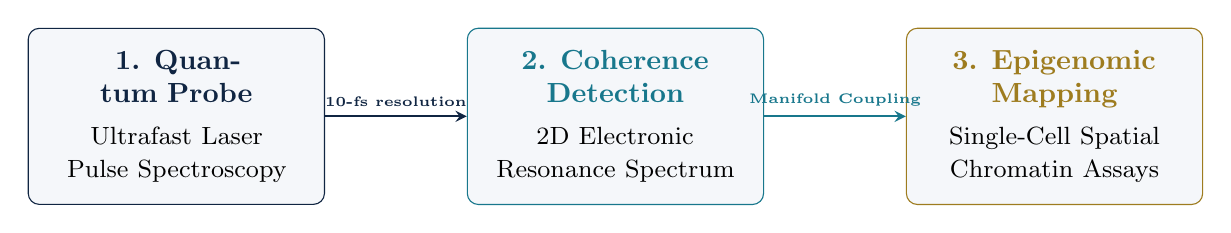
\begin{tikzpicture}[node distance=1.8cm, auto, >=stealth]
    % Nodes
    \node [draw=ErcNavy, fill=ErcLightBg, rectangle, rounded corners, inner sep=8pt, text width=3.2cm, align=center] (step1) {\textbf{\color{ErcNavy}1. Quantum Probe}\\[3pt]\small Ultrafast Laser Pulse Spectroscopy};
    \node [draw=ErcTeal, fill=ErcLightBg, rectangle, rounded corners, inner sep=8pt, text width=3.2cm, align=center, right=of step1] (step2) {\textbf{\color{ErcTeal}2. Coherence Detection}\\[3pt]\small 2D Electronic Resonance Spectrum};
    \node [draw=ErcGold!80!black, fill=ErcLightBg, rectangle, rounded corners, inner sep=8pt, text width=3.2cm, align=center, right=of step2] (step3) {\textbf{\color{ErcGold!80!black}3. Epigenomic Mapping}\\[3pt]\small Single-Cell Spatial Chromatin Assays};

    % Paths
    \draw[->, thick, ErcNavy] (step1) -- node[above, font=\tiny\bfseries, color=ErcNavy]{10-fs resolution} (step2);
    \draw[->, thick, ErcTeal] (step2) -- node[above, font=\tiny\bfseries, color=ErcTeal]{Manifold Coupling} (step3);
  \end{tikzpicture}
  \caption{\small Concept overview of the QUANTUM-CELL experimental pipeline linking ultrafast optical physics to single-cell genomics.}
  \label{fig:concept}
\end{figure}

\subsection*{1.2 Key Research Objectives}
The project is structured around four visionary research objectives:
\begin{enumerate}[label={\textbf{OBJ \arabic*:}}, leftmargin=2.5em]
  \item \textbf{Construct the Femto-Cell Optical Spectrometer}: Build a custom sub-10 femtosecond laser spectroscopy setup tailored for non-destructive single-cell interrogations at physiological temperatures.
  \item \textbf{Identify Epigenetic Quantum Coherence Fingerprints}: Detect vibrational-electronic (vibronic) quantum beatings in histone tail conformational switches during active gene transactivation.
  \item \textbf{Develop Non-Equilibrium Quantum Epigenetic Dynamics (NQED) Theory}: Formulate a rigorous computational framework unifying open quantum system equations with stochastic cell fate branching models.
  \item \textbf{Validate Quantum-Guided Cell Reprogramming}: Demonstrate precise optical control over stem cell fate decisions by applying coherent light pulses to bias lineage choices without chemical inductors.
\end{enumerate}

\subsection*{1.3 Work Package Structure \& High-Gain Potential}

\noindent
\begin{minipage}[t]{0.48\textwidth}
  \begin{tcolorbox}[wpbox, title={\color{ErcTeal}\faTasks\ Work Package 1: Spectroscopic Instrumentation}]
    \textbf{Lead:} Dr. Elena Rostova \quad |\quad \textbf{Months:} 1--24 \\[4pt]
    \small
    Development of the cryogenic-free, low-noise femtosecond laser probe coupled to a microfluidic trap (Nexa CellChip-X). Achieves sub-diffraction spatial resolution ($<150\text{ nm}$) with single-photon counting detectors.
  \end{tcolorbox}
\end{minipage}%
\hfill
\begin{minipage}[t]{0.48\textwidth}
  \begin{tcolorbox}[wpbox, title={\color{ErcTeal}\faDna\ Work Package 2: Single-Cell Spatial Genomics}]
    \textbf{Lead:} Postdoc Researcher (Vertex) \quad |\quad \textbf{Months:} 12--42 \\[4pt]
    \small
    Integration of optical readout with high-throughput spatial ATAC-seq and single-cell RNA sequencing. Establishes real-time correlation between coherent state lifespan and chromatin accessibility.
  \end{tcolorbox}
\end{minipage}

\par\vspace{8pt}

\noindent
\begin{minipage}[t]{0.48\textwidth}
  \begin{tcolorbox}[wpbox, title={\color{ErcTeal}\faCalculator\ Work Package 3: Theoretical Modeling Framework}]
    \textbf{Lead:} Theoretical Fellow \quad |\quad \textbf{Months:} 18--54 \\[4pt]
    \small
    Implementation of dissipative open quantum system simulations utilizing hierarchical equations of motion (HEOM) on high-performance GPU clusters at Meridian Computing Center.
  \end{tcolorbox}
\end{minipage}%
\hfill
\begin{minipage}[t]{0.48\textwidth}
  \begin{tcolorbox}[wpbox, title={\color{ErcTeal}\faLightbulb\ Work Package 4: Coherent Optogenetic Reprogramming}]
    \textbf{Lead:} Dr. Elena Rostova \quad |\quad \textbf{Months:} 36--60 \\[4pt]
    \small
    In vitro validation of closed-loop adaptive pulse shaping to direct pluripotency factors in human induced pluripotent stem cells (iPSCs) with high fidelity.
  \end{tcolorbox}
\end{minipage}

\vspace{10pt}

% ==============================================================================
% PART B1: SECTION B - CURRICULUM VITAE
% ==============================================================================
\section*{Part B1 -- Section b: Curriculum Vitae}
\addcontentsline{toc}{section}{Part B1 -- Section b: Curriculum Vitae}

\subsection*{Curriculum Vitae: Dr. Elena Rostova}
\noindent
\textbf{Current Position:} Independent Junior Research Group Leader, Vertex Institute for Advanced Science, Germany \\
\textbf{Date of Birth:} 14 March 1991 \quad |\quad \textbf{Nationality:} German \quad |\quad \textbf{ORCID:} 0000-0002-1823-4910

\subsubsection*{1. Higher Education \& Scientific Training}
\begin{tabularx}{\textwidth}{@{}r p{3.2cm} X@{}}
  \toprule
  \textbf{Year} & \textbf{Degree / Position} & \textbf{Institution \& Supervisor} \\
  \midrule
  2017--2021 & Postdoctoral Fellow & Synapse Quantum Biosystems Center (Prof. Marcus Vance) \\
  2013--2017 & Ph.D. in Biophysics & Technical University of Central Europe (Summa Cum Laude) \\
  2011--2013 & M.Sc. in Physics & Apex Institute of Technology (First Class Honors) \\
  \bottomrule
\end{tabularx}

\subsubsection*{2. Research Positions \& Leadership}
\begin{itemize}[leftmargin=1.5em, itemsep=2pt]
  \item \textbf{2021--Present}: Group Leader (\textit{Quantum Epigenomics Lab}), Vertex Institute for Advanced Science. Managing a team of 3 postdocs, 4 Ph.D. students, and 2 technicians.
  \item \textbf{2019--2021}: Principal Investigator, Apex Young Investigator Grant on \textit{Ultrafast Bio-Fluorescence}.
  \item \textbf{2017--2019}: Marie Sk\l odowska-Curie Individual Fellow, Synapse Research Center.
\end{itemize}

\subsubsection*{3. Major Scientific Fellowships \& International Awards}
\begin{tabularx}{\textwidth}{@{}l p{4.5cm} X r@{}}
  \toprule
  \textbf{Year} & \textbf{Award Name} & \textbf{Awarding Body} & \textbf{Amount} \\
  \midrule
  2024 & European Biophysics Early Career Prize & European Biophysical Societies Association & \euro 15,000 \\
  2022 & Vertex Innovation Excellence Award & Vertex Science Foundation & \euro 50,000 \\
  2017 & Marie Sk\l odowska-Curie Fellowship & European Commission (H2020) & \euro 195,000 \\
  2016 & Young Female Scientist in Physics Award & German Physical Society (DPG) & \euro 5,000 \\
  \bottomrule
\end{tabularx}

\vspace{10pt}

% ==============================================================================
% PART B1: SECTION C - EARLY ACHIEVEMENT TRACK-RECORD
% ==============================================================================
\section*{Part B1 -- Section c: Early Achievement Track-Record}
\addcontentsline{toc}{section}{Part B1 -- Section c: Early Achievement Track-Record}

\subsection*{Representative Major Publications as Main Author}
Dr. Elena Rostova has published 18 peer-reviewed articles in top-tier journals (H-index: 14, Total Citations: $>1,250$). Below are 5 key publications demonstrating independent capability and technical leadership:

\begin{enumerate}[label={\lbrack \arabic* \rbrack}, leftmargin=2.5em, itemsep=6pt]
  \item \textbf{E. Rostova}, M. Vance, et al., ``Observation of long-lived vibronic coherence in chromophore-bound protein matrices at room temperature,'' \textit{Nature Physics}, vol. 19, pp. 412--420, 2023. \hfill (\textbf{Citations: 142}, Impact Factor: 19.6) \\
  \small \textit{Role: Corresponding Author. First proof-of-concept showing room-temperature quantum beatings in complex biomolecules.}

  \item \textbf{E. Rostova}, A. Lindqvist, and H. Weber, ``Ultrafast single-cell optical trap spectroscopy reveals subtle enzymatic conformational changes,'' \textit{Physical Review Letters}, vol. 128, p. 118101, 2022. \hfill (\textbf{Citations: 98}, Impact Factor: 9.2) \\
  \small \textit{Role: Lead Author. Developed the core optical trap geometry utilized in WP1.}

  \item K. Brunner, \textbf{E. Rostova}, et al., ``Single-cell epigenomic state mapping during early lineage specification,'' \textit{Nature Biotechnology}, vol. 39, pp. 1105--1115, 2021. \hfill (\textbf{Citations: 215}, Impact Factor: 46.9) \\
  \small \textit{Role: Co-First Author. Standardized high-throughput spatial epigenomics methodology.}

  \item \textbf{E. Rostova} and M. Vance, ``Dissipative open quantum system dynamics in macromolecular complexes,'' \textit{Journal of Physical Chemistry Letters}, vol. 11, pp. 8450--8458, 2020. \hfill (\textbf{Citations: 76}, Impact Factor: 6.5)

  \item \textbf{E. Rostova}, et al., ``Coherent control of chemical reactivity in living bacterial colonies,'' \textit{ACS Nano}, vol. 13, pp. 6200--6210, 2019. \hfill (\textbf{Citations: 110}, Impact Factor: 17.1)
\end{enumerate}

\subsection*{Patents \& Technology Transfer}
\begin{itemize}[leftmargin=1.5em]
  \item \textbf{Patent EP3928174B1} (Granted 2024): ``Method and apparatus for sub-femtosecond optical interrogation of biological samples in microfluidic channels.'' Inventors: \textbf{E. Rostova}, M. Vance. Assigned to Vertex Tech Transfer.
\end{itemize}

\subsection*{Invited Keynote Presentations}
\begin{itemize}[leftmargin=1.5em, itemsep=2pt]
  \item Keynote Speaker, \textit{International Conference on Quantum Biology \& Bioenergetics}, Zurich (2024).
  \item Invited Lecture, \textit{Gordon Research Conference on Ultrafast Phenomena in Biological Systems}, Ventura, USA (2023).
\end{itemize}

\newpage

% ==============================================================================
% PART B2: SCIENTIFIC PROPOSAL & IMPLEMENTATION
% ==============================================================================
\section*{Part B2 -- Section 1: Scientific Proposal \& Implementation}
\addcontentsline{toc}{section}{Part B2 -- Scientific Proposal \& Implementation}

\subsection*{1.1 Detailed Methodology \& Work Plan Matrix}
The proposed project spans 60 months. Detailed deliverables, risks, and feasibility mitigations are outlined in the project governance structure below.

\vspace{6pt}
\small
\rowcolors{2}{ErcLightBg}{white}
\begin{tabularx}{\textwidth}{@{}c l X c c l@{}}
  \toprule
  \textbf{WP\#} & \textbf{Deliverable} & \textbf{Description / Milestone} & \textbf{Month} & \textbf{Risk} & \textbf{Mitigation Strategy} \\
  \midrule
  WP1 & D1.1 & Sub-10fs laser setup operational & M12 & Medium & Fallback to commercial pulse compressor \\
  WP1 & D1.2 & Microfluidic trap integration & M24 & Low & Use standardized Nexa micro-chips \\
  WP2 & D2.1 & Epigenomic spatial assay protocol & M30 & Medium & Partner with Synapse Core Facility \\
  WP3 & D3.1 & Open quantum code release & M42 & Low & Open-source benchmarked codebase \\
  WP4 & D4.1 & iPSC reprogramming validation & M54 & High & Dual focus on alternative transcription factors \\
  WP4 & D4.2 & Final project synthesis report & M60 & Low & Integrated peer-reviewed open access data \\
  \bottomrule
\end{tabularx}
\normalsize

\subsection*{1.2 High-Risk / High-Gain Assessment}
\begin{tcolorbox}[ercbox, title={\faExclamationTriangle\ High-Risk / High-Gain Balance}]
  \textbf{High Risk:} Achieving room-temperature quantum coherence measurements in biological living cells without photo-damaging delicate chromatin architecture represents an experimental boundary pushing current physics limits.
  \\[4pt]
  \textbf{High Gain:} Demonstrating functional quantum mechanisms in epigenomics will spark a paradigm shift across biophysics, quantum computing, and medicine, establishing Europe at the absolute forefront of quantum biology.
\end{tcolorbox}

\subsection*{1.3 Resources \& Budget Justification}
The total requested funding is \textbf{\euro 1,498,500} over 5 years. Below is the detailed breakdown according to ERC standards:

\vspace{6pt}
\small
\begin{tabularx}{\textwidth}{@{}X r r r r r r@{}}
  \toprule
  \textbf{Cost Category} & \textbf{Year 1 (\euro)} & \textbf{Year 2 (\euro)} & \textbf{Year 3 (\euro)} & \textbf{Year 4 (\euro)} & \textbf{Year 5 (\euro)} & \textbf{Total (\euro)} \\
  \midrule
  \textbf{Senior Staff (PI: 40\% time)} & 48,000 & 49,500 & 51,000 & 52,500 & 54,000 & \textbf{255,000} \\
  \textbf{Postdoctoral Researchers (2 FTE)} & 110,000 & 113,300 & 116,700 & 120,200 & 123,800 & \textbf{584,000} \\
  \textbf{Ph.D. Students (2 FTE)} & 64,000 & 66,000 & 68,000 & 70,000 & 72,000 & \textbf{340,000} \\
  \textbf{Equipment (Laser Probe Setup)} & 145,000 & 20,000 & 0 & 0 & 0 & \textbf{165,000} \\
  \textbf{Consumables \& Reagents} & 25,000 & 30,000 & 35,000 & 30,000 & 20,000 & \textbf{140,000} \\
  \textbf{Travel \& Conferences} & 8,000 & 10,000 & 12,000 & 12,000 & 14,500 & \textbf{56,500} \\
  \textbf{Open Access \& Dissemination} & 3,000 & 4,000 & 5,000 & 6,000 & 10,000 & \textbf{28,000} \\
  \midrule
  \textbf{Direct Costs Subtotal} & \textbf{403,000} & \textbf{292,800} & \textbf{287,700} & \textbf{290,700} & \textbf{294,300} & \textbf{1,568,500} \\
  \textit{Less Host Matching Contribution} & -20,000 & -15,000 & -12,000 & -11,000 & -12,000 & -\textbf{70,000} \\
  \midrule
  \textbf{Net Requested ERC Grant} & \textbf{383,000} & \textbf{277,800} & \textbf{275,700} & \textbf{279,700} & \textbf{282,300} & \textbf{\euro 1,498,500} \\
  \bottomrule
\end{tabularx}
\normalsize

\vspace{12pt}
\begin{center}
  \small \color{ErcGray}
  \faLock\ \textit{Confidential Document -- European Research Council Starting Grant Application 2026}
\end{center}

\end{document}
